\chapter{Experiments And Observations}
\label{ch:experiments-and-observations}

\section{Simulations and data collection}
\label{sec:running-sim}

The computational model does not formalise any resources to be used to create and run simulations, neither does the model formalise any way to collect data from the simulations.

JUnit is the reference unit test framework for Java, and the basic implementation of the proposed computational model is tested against more than 20 unit tests. However, unit tests also provide the perfect environment to run simulations. If resources such as initial node grid, initial pheromone concentrations and agents are going to be the same for more than one simulation, one can take advantage of test \emph{fixture} with the \emph{@Before} annotation to initialise these objects without repeating code. One could create a class for each simulation with a \emph{Main} method also, however it is more convenient to use the test framework.

Another critical aspect of the simulations is data collection. The model does not describe how data can be acquired during and after the simulation. For the simulations run for this paper logging was used for this purpose. Log4j is a thread-safe logging service maintained by the Apache foundation and it was used throughout the implementation and the simulations. In most of the simulations the logger was setup to write into files that are processed after the simulation is finished. Also, it is possible to configure the logger service to write on the console, so information on the agents can be easily visualised during the execution of the simulations.

\section{Pheromone Concentration Sensitivity}

Due to the model of node selection, agents are very sensitive to the pheromone concentration presented by the environment around them. This happens because the probability of choosing a neighbour node swings from $0\%$ to $100\%$ very swiftly, causing the agents to get trapped.

This experiment investigates how different initial pheromone concentrations in the environment and the amount of pheromone each agent is capable of depositing in each interaction affect the agents navigation through the space. It also has an objective to determine what values of these two parameters are acceptable to use in the other experiments.

Firstly, let's examine the case when all the nodes of the environment are created with no initial concentration of \emph{Forage} pheromone (Figure \ref{fig:initial-a}). When the agent is deciding which node it is going to make the first move to, all neighbours have the same probability of being picked, because of the $0$ of pheromone concentration (Figure \ref{fig:initial-b}). So as it was programmed to, the agent picks one node at random. But before moving to the next node it lays a bit of pheromone, suppose the concentration deposited is $0.1$. When the move is done, the environment around the agent should look like the one pictured in Figure \ref{fig:initial-c}.

\begin{figure}[H]
\myfloatalign
\subfloat[Initial environment]
{\label{fig:initial-a}
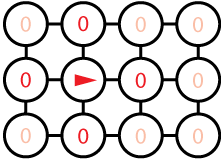
\includegraphics[width=.3\linewidth]{gfx/initial-01}} \quad
\subfloat[Initial probabilities]
{\label{fig:initial-b}
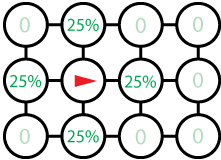
\includegraphics[width=.3\linewidth]{gfx/initial-02}} \\
\subfloat[Environment after move 1]
{\label{fig:initial-c}
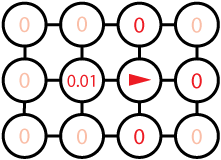
\includegraphics[width=.3\linewidth]{gfx/initial-03}} \quad
\subfloat[Probabilities after move 1]
{\label{fig:initial-d}
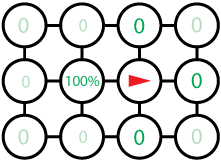
\includegraphics[width=.3\linewidth]{gfx/initial-04}} \\
\subfloat[Environment after move 2]
{\label{fig:initial-e}
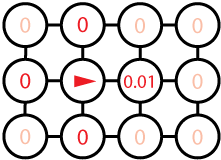
\includegraphics[width=.3\linewidth]{gfx/initial-05}} \quad
\subfloat[Probabilities after move 2]
{\label{fig:initial-f}
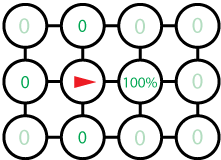
\includegraphics[width=.3\linewidth]{gfx/initial-06}}

\caption{Effect of initial pheromone concentration at zero}\label{fig:initial}
\end{figure}

Now it is time for the agent to move again. Firstly the agent reads the pheromone intensity in each of the neighbour nodes, after it computes where it is more likely to move. For all the nodes around the agent apart from the one it has just moved from have $0$ pheromone intensity in them, the agent is certain to move back to the previous node (Figure \ref{fig:initial-d}). Before completing the move, it lays pheromone in the current node. When the agent is back to the node it first started from, the scenario repeats and it becomes a cycle. The agent go back and forth, trapped in these two nodes forever, with no changes to explore the environment further. 

It is clear that the environment cannot be initialised with no \emph{Forage} pheromone in its nodes. The question that arises from this is: Is there any pair of values for these two parameters that will allow the agents to navigate in an acceptable fashion?

To answer this question, the experiment was setup with the following configuration:

\begin{table}[H]
\myfloatalign
\begin{tabularx}{\textwidth}{Xll} \toprule
\tableheadline{Property} & \tableheadline{Value} \\ \midrule
Number of lines & 500 \\
Number of columns & 500 \\
Total number of nodes &  250,000 \\
\midrule
Duration of each simulation & 10 s \\
Number of agents & 50 \\
Agent Type & WorkerType \\
Task executed & ForageTask \\
Agent sleep time & 5 ms \\
\bottomrule
\end{tabularx}
\caption{Experiment setup for investigation of initial pheromone concentration}  
\label{tab:setup-1}
\end{table}

In Table \ref{tab:setup-1} the property \emph{Agent sleep time} means how long the agent waits after a task is executed to choose another task to run. This is necessary to slow down agents (in this case the threads that are running the agent), otherwise they would cover the entire space in this 10 seconds only by the fact that they can do it very fast not because they are actively foraging.

The initial pheromone concentration and the amount of pheromone deposited in each interaction by the agents were varied from $0.001$ to $0.04$ in $5$ steps. Each of the possible pair of values for the two parameters has been simulated:

\begin{table}[H]
\myfloatalign
\begin{tabularx}{\textwidth}{XXXXX} \toprule
\tableheadline{1} & \tableheadline{2} & \tableheadline{3} & \tableheadline{4} & \tableheadline{5} \\ \midrule
0.001, 0.001 & 0.001, 0.005 & 0.001, 0.01 & 0.001, 0.02 & 0.001, 0.04 \\
0.005, 0.001 & 0.005, 0.005 & 0.005, 0.01 & 0.005, 0.02 & 0.005, 0.04 \\
0.01, 0.001 & 0.01, 0.005 & 0.01, 0.01 & 0.01, 0.02 & 0.01, 0.04 \\
0.02, 0.001 & 0.02, 0.005 & 0.02, 0.01 & 0.02, 0.02 & 0.02, 0.04 \\
0.04, 0.001 & 0.04, 0.005 & 0.04, 0.01 & 0.04, 0.02 & 0.04, 0.04 \\
\bottomrule
\end{tabularx}
\caption{Variations for initial concentration and amount of pheromone deposited by agents}  
\label{tab:setup-2}
\end{table}

In each case, the colony containing $50$ agents is created at the north of the environment, horizontally centred. The agents execute the \emph{ForageTask} since their creation, they do not analyse any contextual parameters such as other agents, they only try to move through the space using the rules defined by the task.

In order to compare how each possible value pairs in Table \ref{tab:setup-2} affect the resulting navigation of the agents, two samples of  the pheromone trail left by the agents are analysed. The first one is from close to the nest that will enable us to check how is the agents' response to the initial pheromone concentration shortly they have left the nest. The second sample is taken further ahead in the environment, far from the nest. This sample is a good way to test how the agents' own deposit of pheromone will affect the system behaviour, Figure \ref{fig:initial-sample} illustrates how and where the samples are made.

\begin{figure}[H]
  \centering
  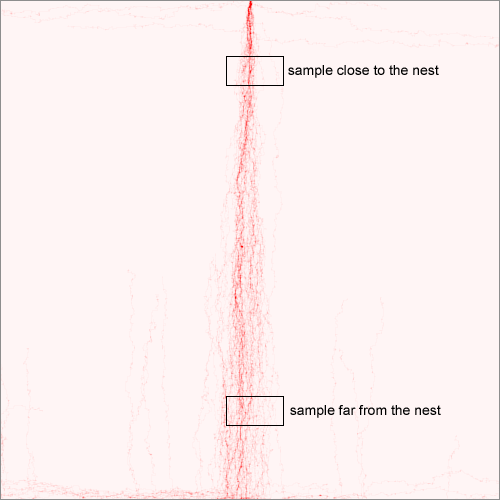
\includegraphics[width=0.4\linewidth]{gfx/initial-sample.png}
  \caption{How the two samples of the environment is made}
  \label{fig:initial-sample}
\end{figure}

Figures \ref{fig:initial-var-close} and \ref{fig:initial-var-far} show the resulting sampling for all possible combination for the initial pheromone concentration and the amount of pheromone deposited by each agent in each interaction.

\begin{figure}[H]
\myfloatalign
\subfloat[]
{\label{fig:initial-var-close}
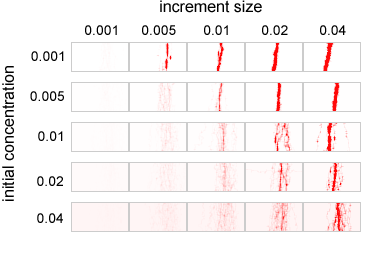
\includegraphics[width=.6\linewidth]{gfx/initial-variations-close}} \\
\subfloat[]
{\label{fig:initial-var-far}
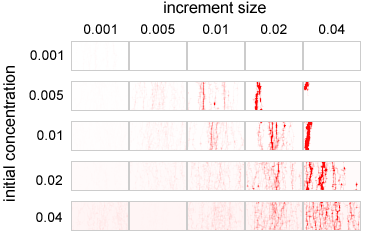
\includegraphics[width=.6\linewidth]{gfx/initial-variations-far}} \\

\caption{Samples of the pheromone trail left by the agents close to the nest (a) and far from the nest (b). }\label{fig:initial-var-final}
\end{figure}


The trails left by the colonies can be compared in relation on how strong they are, how the agents are able to 'scape' them to explore the environment and how it shaped when agents get further from the nest.

Starting from $0.001$ as the amount of pheromone to be deposited by agents in each interaction; it is possible to observe from the figures that two very contrasting behaviours emerge, firstly because the environment has so little pheromone and the update is so small, they weight assigned to each of the neighbour nodes count considerably more than the pheromone deposited by the agents, so the agents end up very dispersed, thus no chemical trail is formed at all. This phenomena is actually seen in many other combination of the parameters, all the cases when the update is $0.001$ in fact. 

When the amount of pheromone deposited by the agents is increased the behaviour of the colony could not be more different than what was seen previously. The agents switch from exploring a large area to be 'trapped' into the pheromone trail. This impedes the agents of exploring the space, what is not desirable for any colony. This behaviour is also seen in other values for the parameters. What seems to be the rule is that if the update is considerable larger than the concentration of pheromone in the environment the agents will start to create a 'bubble' of high pheromone concentration and as consequence they are very unlikely to move to any node outside this area.

It rises the question, why does it happen? The answer is similar to one of the problem in initialising the environment with no pheromone at all. In this case, the critical point is the rate between the initial concentration and the amount deposited by the agents in each interaction.

Figure \ref{fig:update} illustrates how swiftly the probabilities can change depending on the amount of pheromone deposited in the node by agents. The node in red in the picture represents a node that has been updated previously by another agent. In the first scenario (Figure \ref{fig:update-c}) the update was $0.001$, in the second (Figure \ref{fig:update-e}) the pheromone deposited was $0.01$. The probability of the node in red being picked up to be the next node the agent will move to more than doubled. (Figure \ref{fig:update-d} and Figure \ref{fig:update-f}).

\begin{figure}[H]
\myfloatalign
\subfloat[]
{\label{fig:update-a}
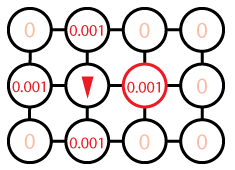
\includegraphics[width=.25\linewidth]{gfx/update-01}} \quad
\subfloat[]
{\label{fig:update-b}
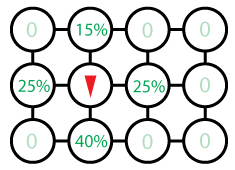
\includegraphics[width=.25\linewidth]{gfx/update-02}} \\
\subfloat[]
{\label{fig:update-c}
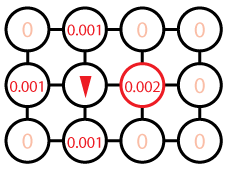
\includegraphics[width=.25\linewidth]{gfx/update-03}} \quad
\subfloat[]
{\label{fig:update-d}
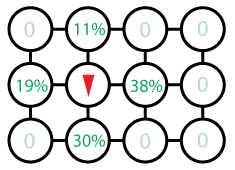
\includegraphics[width=.25\linewidth]{gfx/update-04}} \\
\subfloat[]
{\label{fig:update-e}
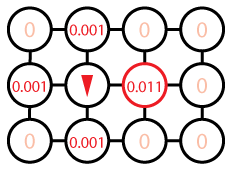
\includegraphics[width=.25\linewidth]{gfx/update-05}} \quad
\subfloat[]
{\label{fig:update-f}
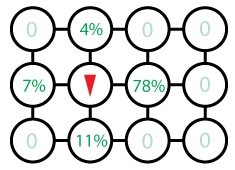
\includegraphics[width=.25\linewidth]{gfx/update-06}}

\caption{Shift of probability depending on agent update}\label{fig:update}
\end{figure}

Further investigation revealed that the probability of selection increases in a logarithmic fashion. Figure \ref{fig:prob-inc} shows how the increase in probability progress when the amount of pheromone deposited by the agents increases by multiples of the initial concentration in the environment.

\begin{figure}[H]
  \centering
  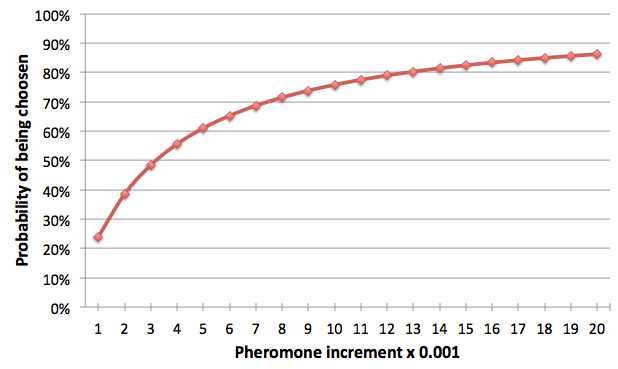
\includegraphics[width=0.6\linewidth]{gfx/probability-increase.png}
  \caption[Selection probability increasing]{Increase of probability selection according to the increase of the deposit increment}
  \label{fig:prob-inc}
\end{figure}

It is very tempting to conclude that if the right ratio between the initial pheromone concentration and the increment step used by the agents is found the, problems of the lack of trail formation and the agent confinement in the trail will be solved. However from figures \ref{fig:initial-var-close} and \ref{fig:initial-var-far} it is observed that the same ratio (initial concentration/increase step) present different results for different values. In the case $0.001/0.001$ no trail is formed at all, for $0.01/0.01$ a solid trail is formed. 

The experimental results are that the initial pheromone concentration should not be too low that avoid trail formation or saturation. It has to be an intermediate value that allows the agents to converge to a specific path, generating the trail, but not too fast, allowing the agents to explore other parts of the environment as well. As far as the update step goes, it also needs to be an intermediate value, so it starts actually being part of the node selection process but not big enough to quickly saturate the pheromone trail.

\begin{figure}[H]
\myfloatalign
\subfloat[]
{\label{fig:trail-a}
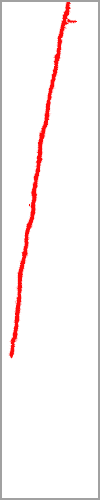
\includegraphics[width=.1\linewidth]{gfx/trail-001}} \quad
\subfloat[]
{\label{fig:trail-b}
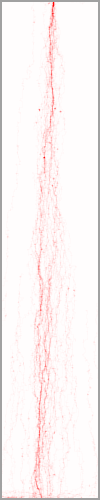
\includegraphics[width=.1\linewidth]{gfx/trail-01}} \quad
\subfloat[]
{\label{fig:trail-c}
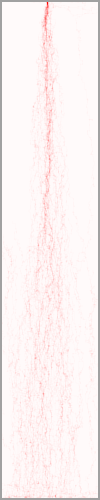
\includegraphics[width=.1\linewidth]{gfx/trail-0201}} \quad
\subfloat[]
{\label{fig:trail-d}
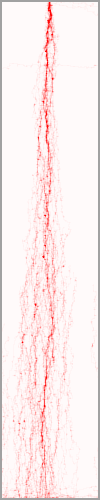
\includegraphics[width=.1\linewidth]{gfx/trail-0202}} \quad
\subfloat[]
{\label{fig:trail-e}
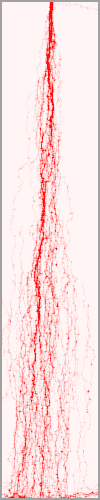
\includegraphics[width=.1\linewidth]{gfx/trail-0404}} \quad

\caption[Example of complete pheromone trails]{Complete trail pheromone trails left by simulation using 0.001,0.04 (a), 0.01,0.01 (b), 0.02,0.01 (c), 0.02,0.02 (d) and 0.4,04 (e) for initial pheromone concentration and update step respectively}
\label{fig:trails}
\end{figure}

One can conclude from this analysis pair $0.01/0.01$ (Figure \ref{fig:trail-b}) for the initial pheromone concentration and increment step present the best results. It allows pheromone trail to \emph{emerge as a result of the agents' interactions with the environment}. It could also be argued that another pairs such $0.01/0.02$ and $0.02/0.02$ set the right conditions for agent navigation. However, in this experiment the agents are executing the \emph{ForageTask} without actually collecting food, to no agent tries to deposit food in the nest and start foraging again - the trail is not reinforced. Taking that in consideration the other pairs tested could also be considered to lead to a premature saturation of the trail, which is the case of $0.02/0.02$.

The pair $0.01/0.01$ also proved to be less sensitive to the number of agents used in this and the other experiments.

\section{Forage Radius Investigation}
\label{sec:forage-radius-inv}

This experiment investigates the affect of the radius variation of the \emph{Forage} chemical stimulus (section \ref{subsec:forage-stimulus}) on the capacity of the colony to collect food. Four values for the stimulus' radius were tried - $0$, $1$, $2$. The experiment was setup as follows:

\begin{table}[H]
\myfloatalign
\begin{tabularx}{\textwidth}{Xll} \toprule
\tableheadline{Property} & \tableheadline{Value} \\ \midrule
Number of lines & 500 \\
Number of columns & 500 \\
Total number of nodes &  250,000 \\
Initial grid pheromone intensity & 0.01 \\
\midrule
Pheromone radius variations & 0, 1, 2 \\
Duration of each simulation & 30 s \\
Number of agents & 50 \\
Agent Type & WorkerType \\
Pheromone increment step & 0.01 \\
Task executed & ForageTask and FindHome\\
Agent sleep time & 5 ms \\
Pheromone decay frequency & every 3 seconds \\
\bottomrule
\end{tabularx}
\caption{Experiment setup for pheromone radius variation study}  
\label{tab:setup-2}
\end{table}

In this experiment the radius of action of the forage pheromone is varied in order to check the effects in the amount of food the colony is capable of forage. At first one would expect that the increase on the radius of the forage pheromone would have a positive impact on the colony capacity of collecting food as trails that lead to food sources would are reinforced by agents caring food back to the nest and with a wider spread of the pheromone more workers would be fall in these trails. However the data from the simulations show a different picture. The colony collect less and less food as the stimulus' radius increase. Table \ref{tab:radius-results} is a summary of the data collected from the study.

For this experiment a row of food sources was placed far away from the colony. Each source has a total amount of food of $30$. The simulation was run $100$ times for each radius variation. Figure \ref{fig:radius-res} presents part of the middle section (see Figure \ref{fig:radius-full-a}) of the trails created by the agents for the first $20$ simulations for each value used for radius.

\begin{figure}[H]
\myfloatalign
\subfloat[radius = 0]
{\label{fig:radius-res-a}
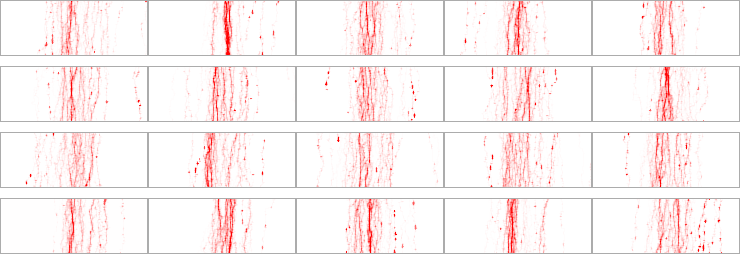
\includegraphics[width=.8\linewidth]{gfx/radius-res-0}} \\
\subfloat[radius = 1]
{\label{fig:radius-res-b}
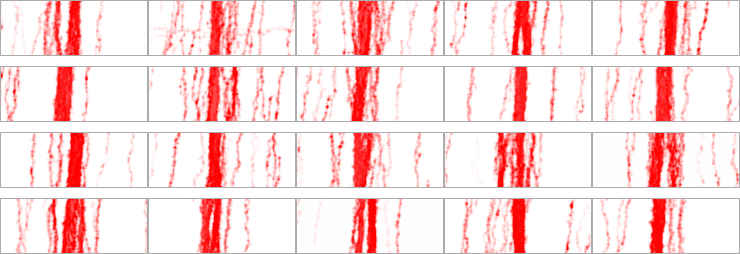
\includegraphics[width=.8\linewidth]{gfx/radius-res-1}} \\
\subfloat[radius = 2]
{\label{fig:radius-res-c}
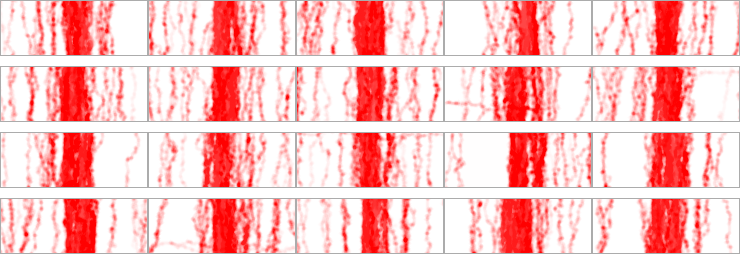
\includegraphics[width=.8\linewidth]{gfx/radius-res-2}} \\

\caption[Visual samples of variation of radius]{20 graphical samples of the results in variating forage stimulus' radius}\label{fig:radius-res}
\end{figure}

\begin{figure}[H]
\myfloatalign
\subfloat[setup]
{\label{fig:radius-full-a}
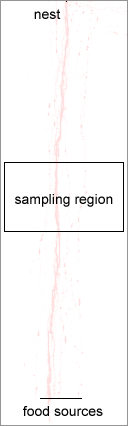
\includegraphics[width=.15\linewidth]{gfx/radius-experiment}} \quad
\subfloat[radius = 0]
{\label{fig:radius-full-b}
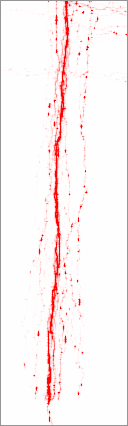
\includegraphics[width=.15\linewidth]{gfx/radius-full-0}} \quad
\subfloat[radius = 1]
{\label{fig:radius-full-c}
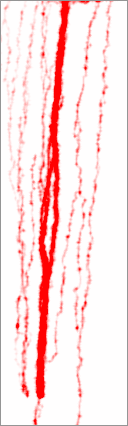
\includegraphics[width=.15\linewidth]{gfx/radius-full-1}} \quad
\subfloat[radius = 2]
{\label{fig:radius-full-d}
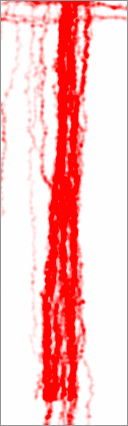
\includegraphics[width=.15\linewidth]{gfx/radius-full-2}}

\caption{Example of trail formation for different radiuses}
\label{fig:radius-full}
\end{figure}

\begin{table}[H]
\myfloatalign
\begin{tabularx}{\textwidth}{Xll} \toprule
\tableheadline{Radius} & \tableheadline{Average of food collected} & \tableheadline{Standard deviation} \\ \midrule
0 & 6.0 & 1.21 \\
1 & 4.9 & 0.72 \\
2 & 3.3 & 0.53 \\

\bottomrule
\end{tabularx}
\caption{Forage radius simulations' outcomes}  
\label{tab:radius-results}
\end{table}

The averages that are presented in the Table \ref{tab:radius-results} was calculated after statistically validating the dataset collected for each radius value, with any outlier sample was removed from the results collected from the simulations. The following pair of equation are used to define a sample point $x_i$ as outlier or not:

\begin{equation}
\begin{cases} 

x_{i} \leq \bar{x} - 2 \times \sigma \\
x_{i} \geq \bar{x} + 2 \times \sigma

\end{cases}
\end{equation}

Where $\bar{x}$ is the average of the resulting dataset for each radius and $\sigma$ is the standard deviation. The data collected proved to be consistent and only few samples were rejected. Figure \ref{fig:radius} shows the samples spread for each radius and their probability density distribution.

\begin{figure}[H]
\myfloatalign
\subfloat[]
{\label{fig:radius-a}
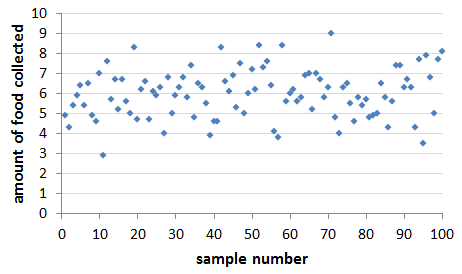
\includegraphics[width=.4\linewidth]{gfx/radius-0}} \quad
\subfloat[]
{\label{fig:radius-b}
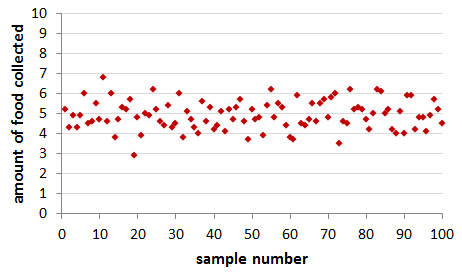
\includegraphics[width=.4\linewidth]{gfx/radius-1}} \\
\subfloat[]
{\label{fig:radius-c}
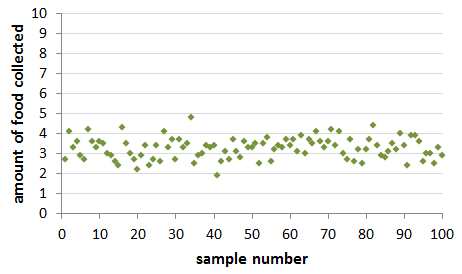
\includegraphics[width=.4\linewidth]{gfx/radius-2}} \quad
\subfloat[]
{\label{fig:radius-d}
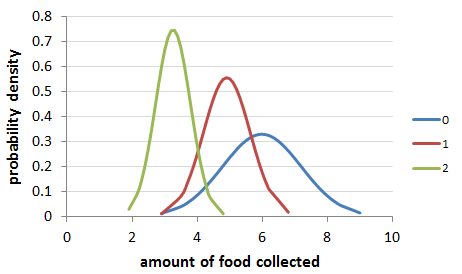
\includegraphics[width=.4\linewidth]{gfx/radius-pdf}}

\caption[Radius variation - samples distributions]{Samples distribution variating the pheromone radius - 0 (a), 1 (b) and 2 (c) - and the samples' probability density distribution (d)}\label{fig:radius}
\end{figure}

Figure \ref{fig:radius} helps to visualise what the standard deviations from Table \ref{tab:radius-results} had already shown - the samples \emph{variance} decreases when the radius increases. The reason for this phenomena is that the bigger the pheromone radius is the lesser agents are probable to 'escape' from the trail, thus they are not able to explore different areas of the environment. For the agents use virtually only the same pheromone trail to forage their outcomes are likely to be very close.  

With a more diversified exploratory reach, agents in the simulations using radius $0$ are likely to have different degrees of success in finding food and taking it back to the nest in each simulation run, justifying the greater variance in the colony outcome.

The study carries raises another question - why does smaller radiuses outperform bigger ones? From Table \ref{tab:radius-results} we can see that the simulations with radius $0$ outperforms the ones with radiuses $1$ and $2$ in $22$ and $82$ percent in average respectively. This occurs due to the formation of trails with large width, leading the agents to move from note to node in almost random fashion. 

Figure \ref{fig:radius-res} illustrates how the pheromone trails widen with the increase of the pheromone radius. It might seem contradictory at first that wider trails do not led to better forage performance, for more ants should be lead to food sources. However due to the model of node selection implemented the agents are too sensitive to the pheromone intensity of the direct neighbours of the node they are currently at, and this is translated to random node selection when agents are trapped in wide pheromone trails. 

\begin{figure}[H]
\myfloatalign
\subfloat[]
{\label{fig:radius-sat-a}
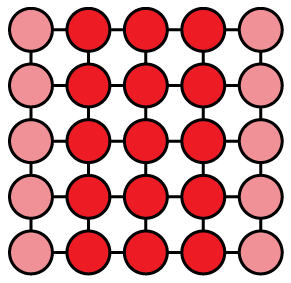
\includegraphics[width=.3\linewidth]{gfx/radius-sat}} \quad
\subfloat[]
{\label{fig:radius-sat-b}
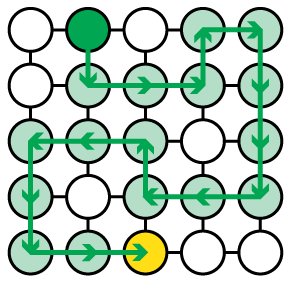
\includegraphics[width=.3\linewidth]{gfx/radius-sat-nav}}

\caption{Affect of wide pheromone trails on node selection}\label{fig:radius-saturation}
\end{figure}

This random behaviour, as far node selection is concerned, has a profound impact on the colony's forage performance, as agents will struggle to find their way to the food sources, and when eventually some of them do, there still a good change that many will not reach the nest back in order to deposit the food they have collected.  

This strongly suggests that ants use more than only local information available at the instant they are making decision where to move to. The other communication methods employed by ants should play a vital role in assisting this decision to be made.

Figure \ref{fig:radius-explored} is a renderisation  of the space visited by all ants of the colony throughout the simulation (left frame) and the space visited by only one of the agents of that colony (right frame), set to be tracked by the framework. As it is possible to see, as the radius increases so does the number of paths the agents visit and more tortuous they become. Figures \ref{fig:radius-exp-b} and \ref{fig:radius-exp-c} also show how the ants get 'trapped' in the pheromone cloud. In both figures, the paths formed by the single agent (right frame) have the same shape of the main stream of paths visited by the entire colony (left frame). 


Two new possible experiments to better understand and improve node selection are proposed in section \ref{sec:new-studies}.

\begin{figure}[H]
\myfloatalign
\subfloat[]
{\label{fig:radius-exp-a}
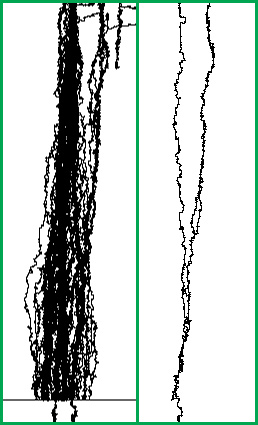
\includegraphics[width=.25\linewidth]{gfx/radius-explored-0}} \quad
\subfloat[]
{\label{fig:radius-exp-b}
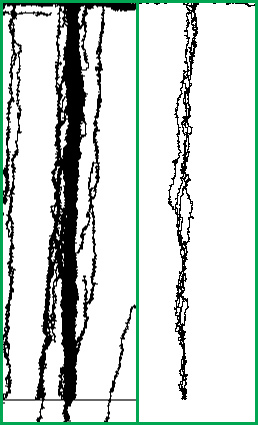
\includegraphics[width=.25\linewidth]{gfx/radius-explored-1}} \quad
\subfloat[]
{\label{fig:radius-exp-c}
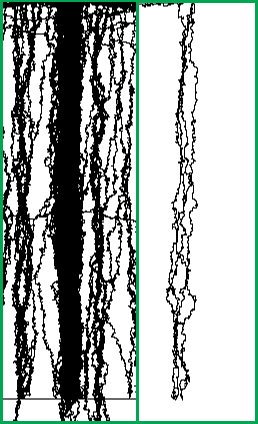
\includegraphics[width=.25\linewidth]{gfx/radius-explored-2}}

\caption{Examples of the space explored by the entire colony (left) and by one agent only (right). Varying the stimulus' radius form $0$ (a) and $1$ (b) to $2$ (c).}\label{fig:radius-explored}
\end{figure}

%\section{Warning Pheromone Response}
%\label{sec:warn-phero-inv}
%In this experiment the response of the agents to a warning communication stimulus is tested.

%Describe the experiment setup.

%Explain that the experiment is done in two phases, the first one the agents react only to amount of warning pheromone and the second one the agents react also to the number of other agents they meet that are traveling in the opposite direction and are not caring food.

%Add block diagrams that explain the algorithms the agents use to decide on task selection.

%Discuss the results. [experiment not done yet]
%Results should vary with the use of different parameters, such as the number of agents traveling in the opposite direction before the agent abort the current task and change to findNestAndHide task.
